\section{What Terminal Currents Add to Voltage Signatures}
\label{sec:channel-information}

This diagnostic compares the observation sets available to distinguish
fixed source responses. It uses the nominal switched predictor and its
implemented terminal map, including the provisional bus-5 assignment.
Loads have a fixed 10\% change; lines use their opening operators without
an adjustable amplitude. The onset and pre-event state are supplied.
These are model-based separations, not attribution outcomes of the
sequential detector.

\paragraph{A common temporal noise reference.}
To compare nested observation sets, all source means share one reference
covariance. The quiet no-intervention predictor defines
\begin{align}
 r_k&=J_0 m_k+e_k,\\
 m_{k+1}&=T_0m_k+K_0e_k,
 \qquad e_k\sim\mathcal N(0,S_0),
\end{align}
with independent innovations and fixed initial predictive state.
Here $m_k$ is the predictor's conditional mean, rather than a new
physical plant state. Stacking reports gives
$\Sigma=L(I\otimes S_0)L^\top$, where $L$ has identity diagonal blocks and
$L_{kr}=J_0T_0^{k-r-1}K_0$ for $k>r$.
Thus selecting voltage and current coordinates retains the induced
cross-time covariance. It is not equivalent to selecting coordinates
from innovations produced by a filter that already used all channels.

\paragraph{Conditional separation.}
Let $d$ be the difference between two fixed mean trajectories. Partition
the selected report coordinates into voltage $V$ and current $I$ and set
\begin{align}
 S_{I\mid V}&=\Sigma_{II}-\Sigma_{IV}\Sigma_{VV}^{-1}\Sigma_{VI},\\
 d_{I\mid V}&=d_I-\Sigma_{IV}\Sigma_{VV}^{-1}d_V.
\end{align}
For a positive-definite common covariance,
\begin{align}
 Q_{VI}&=Q_V+Q_{I\mid V},\\
 Q_V&=\tfrac12d_V^\top\Sigma_{VV}^{-1}d_V,\\
 Q_{I\mid V}&=\tfrac12d_{I\mid V}^\top S_{I\mid V}^{-1}d_{I\mid V}.
\end{align}
The second term is nonnegative and measures the contribution of current
coordinates after conditioning on voltage for this pair. It is a
standard Gaussian identity. It does not establish the contribution
of currents after separately fitting severity or other nuisance
parameters, and it does not decompose the actual bank's model-dependent
likelihoods. The nearest competing source may also change with the
observation set.

\paragraph{Executed calculation.}
The operators and quiet covariance come from one nominal calibration
bank built with a 300-report PMU prefix. No test outcomes were used.
We evaluated all 153 unordered source pairs at horizons of 3, 15 and
30 reports (0.1, 0.5 and 1\,s at 30 reports/s); the stored table includes
both directions. These are deterministic comparisons, not independent
event replicates. At 1\,s the ratio of minimum pairwise separation with
V+I to that with V has median $\ChannelGainMedian$ and range
$\ChannelGainMin$--$\ChannelGainMax$ across sources.
For each source's nearest V+I competitor, the conditional current term
accounts for a median \ChannelCurrentShareMedian\% of joint separation,
with range \ChannelCurrentShareMin\%--\ChannelCurrentShareMax\%.
The two summaries answer different questions: the first permits the
nearest competitor to change; the second holds the compared pair fixed.

\begin{figure*}[t]
\centering
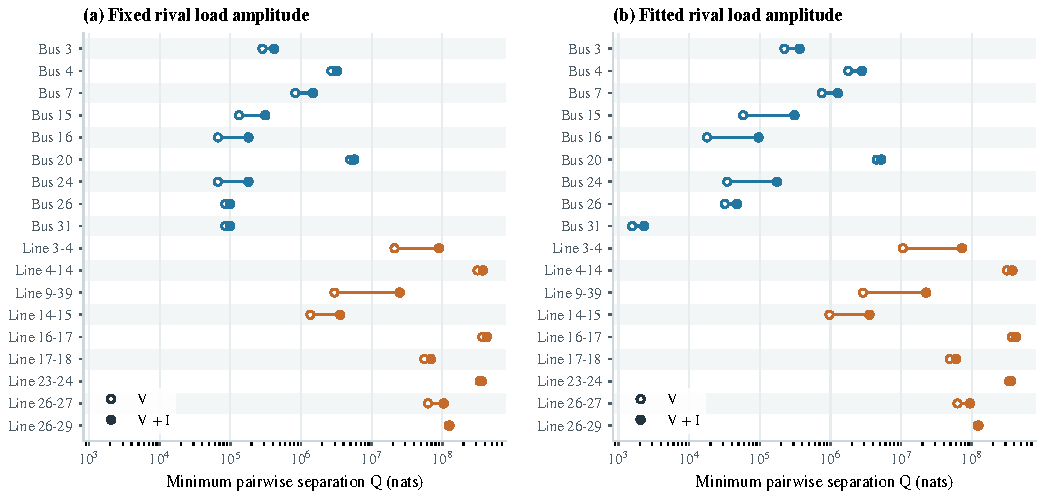
\includegraphics[width=.97\textwidth]{figures/generated/channel_profile_information.pdf}
\caption{Terminal-current information under a common nominal covariance
at 1\,s. Blue denotes load changes and orange line openings.
(a) Minimum fixed-amplitude pairwise separation using voltage alone
(open circles) or voltage and current (filled circles); the minimizing
competitor may differ. (b) Rival load amplitudes are fitted over
$[-0.2,0.2]$, while line openings retain their fixed operators.
Onset, initial state and true source amplitudes are fixed in both
panels; these values do not measure detector performance.}
\label{fig:channel-information}
\end{figure*}

The implementation reconstructs the raw-report covariance recursively
and checks it against an explicit innovation transformation. Their
relative discrepancy is below $6\times10^{-16}$ at three reports.
Full-channel quadratic forms agree with the null-innovation calculation
to $3.1\times10^{-15}$ relative error over all pairs and horizons;
the conditional decomposition agrees to $1.4\times10^{-11}$.
All nested-channel distances are nondecreasing. The source package
contains the compact operator snapshot, channel maps, checksums,
calculation and figure-generation scripts.

\paragraph{Allowing a rival to fit severity.}
For a load rival with mean $\mu_j(b)=o_j+s_jb$, set
$d=\mu_i-o_j$. Under the same common covariance, its best bounded fit is
\begin{equation}
 b^*=\operatorname{clip}_{[-0.2,0.2]}
 \frac{s_j^\top\Sigma^{-1}d}{s_j^\top\Sigma^{-1}s_j},
 \qquad s_j\ne0.
\end{equation}
The profiled separation is
$\widetilde Q_{i\mid j}=\tfrac12\|d-s_jb^*\|_{\Sigma^{-1}}^2$.
Line rivals retain their complete opening trajectories, with no fitted
amplitude. This is deterministic profiling, not integration of the
truncated severity prior used by the detector.

For each common feasible amplitude $b$, the conditional decomposition
gives $Q_{VI}(b)=Q_V(b)+Q_{I\mid V}(b)\ge Q_V(b)$. Hence
$\min_bQ_{VI}(b)\ge\min_bQ_V(b)$. This does not imply that the two
separately minimized terms add to the joint minimum: both must use the
same amplitude. The inequality also holds after minimizing over the
same rival catalog, although the nearest rival may change.

We repeated all source comparisons with bounded rival load severity,
keeping true load changes at 10\% and the same covariance and horizons.
Every analytic load fit agreed with an independent scalar numerical
optimizer to relative error below $10^{-12}$. At 1\,s, the ratio of
minimum V+I to V separation has median $\ProfileChannelGainMedian$
and range $\ProfileChannelGainMin$--$\ProfileChannelGainMax$.
With V+I, \ProfileChannelNearestChanges{} sources change their nearest
rival after fitting severity. The bus-31 source retains only
\ProfileChannelBusThirtyOneRetained\% of its fixed-amplitude minimum
separation: its nearest rival changes from bus~26 to bus~7.
Thus a large distance between fixed responses can conceal ambiguity
between source and magnitude. These nominal comparisons do not establish
how often that ambiguity causes an attribution error.

\paragraph{Interpretation.}
The reference covariance is fixed across sources; candidate-specific
covariance terms, uncertain onset, severity marginalization, pruning,
publication thresholds and false alarms are outside this diagnostic.
The full set contains 16 voltage, 15 current and 16 frequency/ROCOF
coordinates. Those derivative coordinates follow the implemented
measurement model; their incremental separation is not a statement
about independent physical sensors. An empirical channel ablation
would require rebuilding each filter with its own observed coordinates
and calibrating its publication rule before a new independent test.
